% begin module linearization-ex1
\begin{frame}
\begin{example} %[Example 1, p. 241]
Find the linearization of the function $f(x) = \sqrt{x+3}$ at $\alertNoH{9}{a = 1}$ and use it to approximate the numbers $\sqrt{3.98}$ and $\sqrt{4.05}$.  Are these approximations overestimates or underestimates?
\begin{columns}[c]
\column{.5\textwidth}
\begin{itemize}
\item<2-| alert@3-4>  $f'(x) = \fcAnswerUncover{2 }{4}{\frac{1}{2\sqrt{x+3}}.}$
\item<2-| alert@5-6,12>  $f(1) = \fcAnswerUncover{2 }{6}{\sqrt{1+3} = 2.}$
\item<2-| alert@7-8,14>  $f'(1) = \fcAnswerUncover{2 }{8}{\frac{1}{2\sqrt{1+3}} = \frac{1}{4}.}$
\item<2->  Linearization:
\end{itemize}
\abovedisplayskip=0pt
\belowdisplayskip=0pt
\abovedisplayshortskip=0pt
\belowdisplayshortskip=0pt
\begin{align*}
\uncover<9->{%
L(x)&  = \fcAnswerUncover{9}{12}{2} + \fcAnswerUncover{9}{14}{\frac{1}{4}}(x- \fcAnswer{10}{1})
}\\%
& \uncover<15->{ = \frac{7}{4} + \frac{x}{4}}%
\end{align*}
\column{.5\textwidth}
\psset{xunit=0.6cm, yunit=0.6cm}
\begin{pspicture}(-5, -5)(5,5)
\tiny
\psframe*[linecolor=white](-5,-5)(5,5)
\psaxes[ticks=none, labels=none]{<->}(0,0)(-4,-0.5)(5,3.5)
%Function formula: sqrt{}(3+x)
\psline(-3, -0.1)(-3, 0.1)
\rput[t](-3, -0.15){$-3$}
\psline(1, -0.1)(1, 0.1)
\rput[t](1, -0.15){$1$}
\rput(3.5,2){$y=\sqrt{3+x}$}
\psplot[linecolor=red, plotpoints=1000]{-3}{5}{x 3 add sqrt }
\fcFullDotBlack{1}{2}
\rput[b](1,2.1){$(1,2)$}
%Function formula: 7/4+1/4 (x)
\uncover<15->{
\rput(-2,2){$y=\frac74+\frac14 x$}
\psplot[linecolor=blue, plotpoints=1000]{-4}{5}{x 0.25 mul 1.75 add }
}
\end{pspicture}
%\ \only<handout:0| -11>{%
%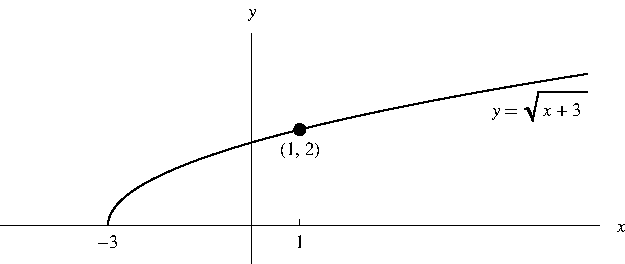
\includegraphics[width=6cm]{differentials/pictures/03-09-ex1a.pdf}%
%}%
%\only<12->{%
%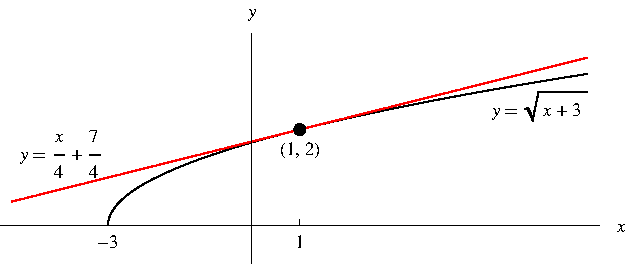
\includegraphics[width=6cm]{differentials/pictures/03-09-ex1b.pdf}%
%}%

\uncover<21->{%
The graph of the linearization is above the curve, so these are overestimates.%
}%
\end{columns}
\begin{itemize}
\item<16-| alert@17-18>  $\sqrt{3.98} = f(0.98) \approx \fcAnswerUncover{16}{18}{\frac{7}{4} + \frac{0.98}{4} = 1.995.}$
\item<16-| alert@19-20>  $\sqrt{4.05} = f(1.05) \approx \fcAnswerUncover{16}{20}{\frac{7}{4} + \frac{1.05}{4} = 2.0125.}$
\end{itemize}
\end{example}
\end{frame}
% end module linearization-ex1
